\section{State of the Art}
Die Teilschritte einer verlustbehaftete Kompressionen können in drei Verarbeitungsarten eingeteilt werden: Transformationen, Quantisierungen und Entropie Kodierungen. Die Abbildung \ref{state:aufbau} zeigt eine vereinfachte Abfolge. Die Inputdaten werden durch ein oder mehrere Verfahren transformiert. Die Transformationen haben das Ziel die Daten so aufzubereiten, dass die folgende Quantisierungen unwichtige Informationen löschen können. Die Transformationen sind meistens verlustfrei umkehrbar, sodass nur in den Quantisierungsschritten Informationen gelöscht werden. Die reduzierte Information wird Entropie Kodiert. Die Entropie Kodierung ist typischerweise für die Datenreduktion verantwortlich.\\
\begin{figure}[!htbp]
	\center
	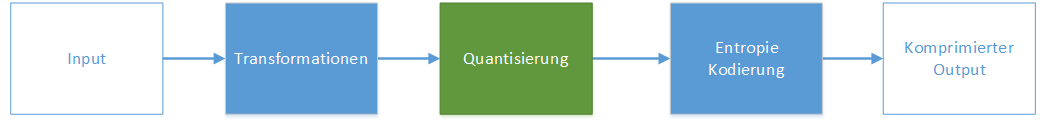
\includegraphics[width=0.8\textwidth,height=6cm,keepaspectratio]{./pictures/state/aufbau.png}
	\caption{Vereinfachter Ablauf einer verlustbehafteten Kompression}
	\label{state:aufbau}
\end{figure}

\subsection{JPEG/JFIF Bildkompression}
\begin{figure}[!htbp]
	\center
	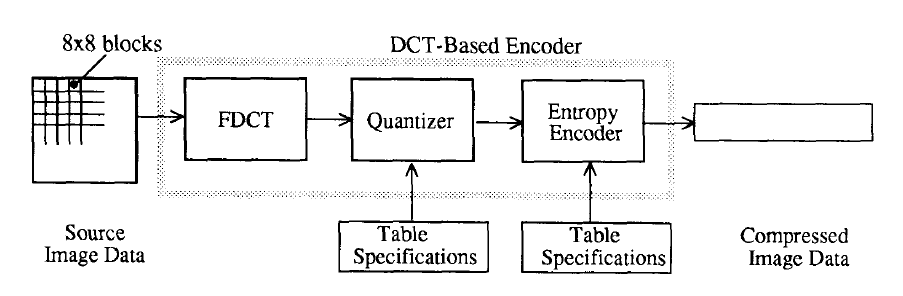
\includegraphics[width=0.8\textwidth,height=6cm,keepaspectratio]{./pictures/state/jpeg.png}
	\caption{Aufbau der JPEG Kompression \cite{wallace1992jpeg}}
	\label{state:jpeg:abb}
\end{figure}
Der JPEG/JFIF Standard ist eines der meist verwendeten Bildkompressionsalgorithmen für natürliche Bilder. Das Diagramm der Abbildung \ref{state:jpeg:abb} zeigt den Aufbau der Kompressionspipeline. JPEG/JFIF unterteilt das Eingabebild in $8*8$ Blöcke und führt eine Diskrete Kosinus Transformation (DCT) durch. Der Bildblock ist nun als Folge von Kosinus Funktionen dargestellt.\\
Die Quantisierung versucht nun Frequenzen, welche das menschliche Auge schlecht erkennen kann weniger Präzise darzustellen. Wenn die Quantisierung gut gewählt wurde, kann der Mensch das dekomprimierte Bild nicht vom Original unterscheiden, verbraucht aber weniger Speicherplatz. JPEG/JFIF bietet vorgefertigte Quantisierungstabellen an. Der Benutzer kann aber eigene Tabellen für spezifizieren. Wie die Quantisierungstabelle optimal gewählt wird, ist ein aktives Forschungsfeld \cite{wu1993rate:jpeg} \cite{wang2001designing:jpeg} und kann von Anwendungsfall zu Anwendungsfall unterschiedlich sein.\\
Nach der Quantisierung werden die quantisierten Blöcke im Zick-Zack-Muster angeordnet, sodass die Entropie Kodierung eine bessere Kompression durchführen kann. JPEG/JFIF führt eine Run-Length\cyte{wiki:rle} und eine Huffman-Kodierung\cite{huffman1952method} durch. JPEG bietet auch hier an, eine benutzerspezifizierte Huffman-Tabelle zu verwenden.

Wenn für die Kompression von wissenschaftlichen Daten eine Diskrete Kosinus Transformation eingesetzt werden soll, kann ein ähnlicher Aufbau verwendet werden wie der JPEG/JFIF Strandard. Für eine optimale Kompression wird die Umsetzung der einzelnen Schritte vom Standard abweichen.

\subsection{Point Cloud Kompression} \label{state:pointcloud}
\begin{figure}[!htbp]
	\center
	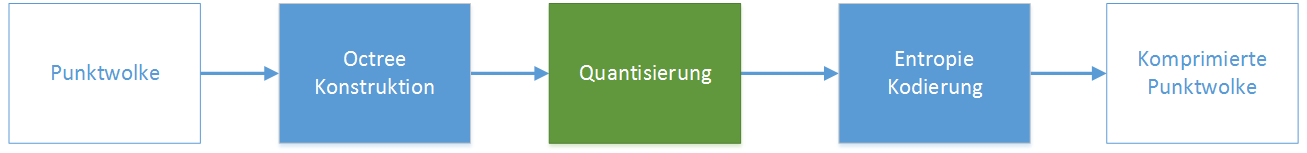
\includegraphics[width=0.8\textwidth,height=6cm,keepaspectratio]{./pictures/state/pointcloud.png}
	\caption{Aufbau einer Octree basierten Point Cloud Kompression.}
	\label{state:pointcloud:abb}
\end{figure}
3d Laser Sampling Geräte produzieren grosse Mengen an dreidimensionalen Punkten von alltäglichen Objekten. Die Kompression von solchen Punktwolken ist ein aktives Forschungsfeld. Eine vorgeschlagene Kompression  von Schnabel und Klein \cite{schnabel2006octree} verwendet Octrees \cite{wiki:octree}. Das Diagramm der Abbildung \ref{state:pointcloud:abb} verdeutlicht den Ablauf.\\
Die dreidimensionalen Punkten werden in einem Octree mit einer begrenzten Anzahl an Levels abgelegt. Im Quantisierungsschritt werden die Punkte durch die Zellenmittelpunkte des Octrees ersetzt. Die Anzahl an Levels ist gleichzusetzen mit der Genauigkeit in Bits welche für jede Koordinatenachse zur Verfügung stehen. Wenn die Levels auf $8$ begrenzt sind, steht für jede Achse $8$ Bit Genauigkeit zur Verfügung.\\
In der Entropie Kodierung wird der Octree zuerst Binär abgebildet ($0$ für leere Knoten, $1$ für befüllte Knoten) in Breadth-First Ordnung. Jedes Level im Octree stellt eine Approximation der Punktwolke dar. Durch die Breadth-First Ordnung werden die ungenaueren Approximationen zuerst abgelegt. Diese Eigenschaft wird mit einer Prediktiven Kodierung ausgenutzt: Aus den vorhergehenden Levels wird eine Vorhersage erstellt, wie die Punkte im nächsten Level zu liegen kommen. Die Kodierung kann die Information reduzieren, indem nur noch der Fehler der Kodierung abgespeichert wird. Je besser die Kodierung das Verhalten vorhersagen kann, desto besser ist die Kompression.

Für diesen Ansatz muss zu einem die Information, welcher Punkt zu welcher Linie gehört, gespeichert werden. Jedem Punkt kann eine Farbe zugewiesen werden. Die Farbe könnte man brauchen um die Punkte den Feldlinien zuzuordnen. Weiter müsste vermutlich die Prediktive Kodierung angepasst werden: Schnabel und Klein nehmen an, dass die Punktwolke eine Oberfläche darstellen. Die Feldlinien jedoch bilden im Allgemeinen keine Oberfläche und benötigen deshalb eine andere Prediktive Kodierung.

\subsection{Curve Fitting}
Curve Fitting ist ein Prozess, welcher ein Signal durch eine oder mehrere Funktionen abbildet. Es ist dabei zwischen einem exakten Curve Fitting und einer Approximation zu unterscheiden. Die exakte Repräsentation wird typischerweise für die Signalinterpolation verwendet, wäherend eine Approximation in der Rauschunterdrückung zum Einsatz kommt. Eine Datenkompression ist mit Curve Fitting möglich, wenn die Parameter der approximierenden Funktion weniger Speicherplatz benötigen, als das Signal.\\
Unser et al \cite{unser1993b:spline} zeigt ein Algorithmus, welcher ähnlich die Diskrete Kosinus Transformation ein diskretes Signal als Folge von B-Splines darstellt. Es wird aufgezeigt, wie eine verlustbehaftete Bildkompression mittels B-Splines möglich ist. Der Vorteil der B-Splines ist, dass die Artefakte der Dekompression als Rauschunterdrückung und Schärfung des Originalbildes ausdrücken.

Eine Datenkompression mit Curve Fitting ist im Vergleich mit der Kosinus Transformation weniger erforscht. Es sind ebenfalls keine Kompressionsstandards bekannt, welche ein Curve Fitting für die Datenkompression verwenden. Ein Kompressionsverfahren zu entwickeln zieht zusätzlichen Aufwand mit sich als Verfahren, welche in der Datenkompression etabliert sind.

\subsection{Compressive Sensing}
Compressive Sensing ist ein Verfahren aus der Signalverarbeitung \cite{baraniuk2007compressive}.
Underdetermined linear system?

\subsection{Entropie Kodierung}
Die Entropie Kodierung findet in allen Bereichen der Informatik Anwendungen. Ziel ist es die gleiche Information mit einem Minimum an Daten darzustellen. Verlustbehaftete Kompressionsverfahren reduzieren die Information und verwenden im letzten Schritt eine Entropie Kodierung um die Datenmenge zu reduzieren.

Es ist zwischen spezialisierten und allgemeinen Entropie Kodierer zu unterscheiden. Unter den spezialisierten Verfahren ist Beispielswiese die Arbeit von Ratanaworabhan et al.\cite{ratanaworabhan2006fast} einzuordnern, welche in der Lage ist Floating Point Daten performant zu kodieren und dekodieren. 
Unter den allgemeinen Verfahren sind Archivierer wie GZIP\cite{website:gzip}, 7-ZIP\cite{website:7zip} und RAR\cite{website:rar} angesiedelt.\\ Archivierungsverfahren finden in allen Bereichen Anwendung und dienen in der Entwicklung von spezialisierten Kodierer als Messbasis. Im Vorfeld wurde die Kompressionsraten von GZIP, 7-ZIP und RAR von Feldliniendaten gemessen. Die Entropie Kodierung von RAR konnte stets eine höhere Kompressionsrate erreichen als andere Archivierungsverfahren. Die RAR Kompression ist urheberrechtlich Geschützt und die verwendeten Algorithmen sind nicht bekannt. 

Es verwendet aber für unterschiedliche Datentypen unterschiedliche Verfahren